\documentclass{article}
\usepackage[a4paper, margin=2cm]{geometry}
\usepackage{tikz}
\usetikzlibrary{arrows.meta, bending}
\usepackage{xcolor}

% Inline event-mention box — identical to the reference template
\newcommand{\tikzmarkbox}[3][]{%
  \tikz[remember picture, baseline=(#2.base)]%
    \node[
      draw=blue,
      fill=blue!10,
      rectangle,
      rounded corners,
      inner sep=1pt,
      outer sep=0pt,
      #1,
      anchor=base
    ] (#2) {#3};%
}

\parindent=0pt
\begin{document}

\begin{figure}[htbp]
\centering

{\normalsize\bfseries EventStoryLine~0.9\enspace$\cdot$\enspace\texttt{3\_7ecbplus.xml}}

\medskip

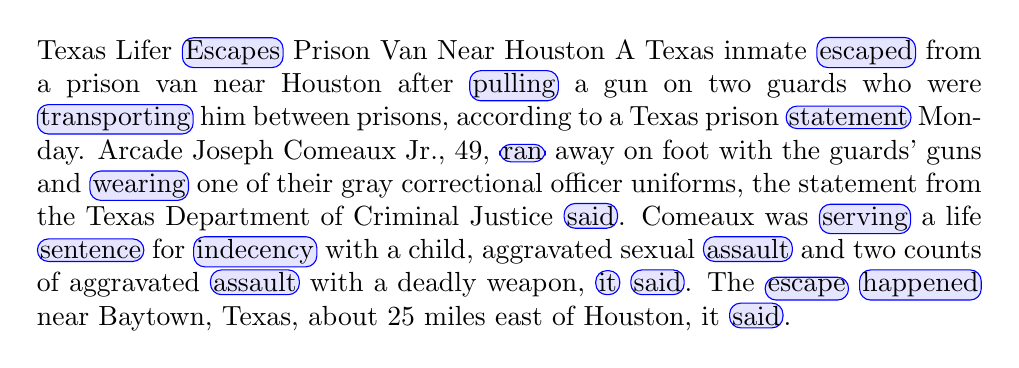
\begin{tikzpicture}[remember picture]
\node[text width=12.0cm, align=justify] (mainText) {%
Texas Lifer \tikzmarkbox{n1}{Escapes} Prison Van Near Houston A Texas inmate \tikzmarkbox{n2}{escaped} from a prison van near Houston after \tikzmarkbox{n3}{pulling} a gun on two guards who were \tikzmarkbox{n4}{transporting} him between prisons, according to a Texas prison \tikzmarkbox{n34}{statement} Monday. Arcade Joseph Comeaux Jr., 49, \tikzmarkbox{n5}{ran} away on foot with the guards' guns and \tikzmarkbox{n6}{wearing} one of their gray correctional officer uniforms, the statement from the Texas Department of Criminal Justice \tikzmarkbox{n15}{said}. Comeaux was \tikzmarkbox{n7}{serving} a life \tikzmarkbox{n8}{sentence} for \tikzmarkbox{n9}{indecency} with a child, aggravated sexual \tikzmarkbox{n10}{assault} and two counts of aggravated \tikzmarkbox{n11}{assault} with a deadly weapon, \tikzmarkbox{n12}{it} \tikzmarkbox{n16}{said}. The \tikzmarkbox{n13}{escape} \tikzmarkbox{n14}{happened} near Baytown, Texas, about 25 miles east of Houston, it \tikzmarkbox{n17}{said}.%
};
\end{tikzpicture}

\medskip

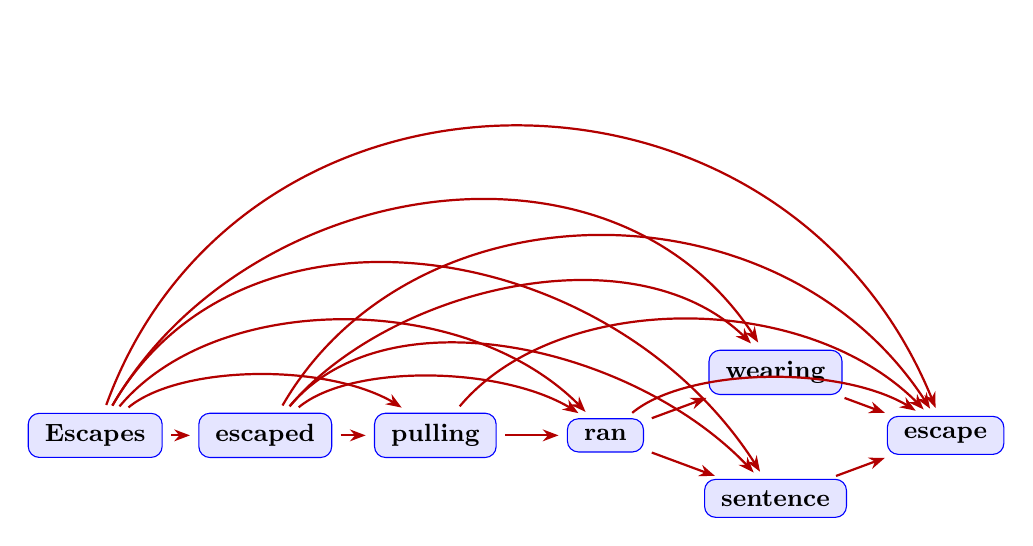
\begin{tikzpicture}[
  event/.style={draw=blue, fill=blue!10, rounded corners,
    inner xsep=6pt, inner ysep=4pt, font=\small\bfseries},
  causes/.style={-{Stealth[length=2mm]}, thick, red!70!black, shorten <=3pt, shorten >=3pt}
]
  \node[event] (n1) at (0.6, 0.0) {Escapes};
  \node[event] (n2) at (2.76, 0.0) {escaped};
  \node[event] (n3) at (4.92, 0.0) {pulling};
  \node[event] (n5) at (7.08, 0.0) {ran};
  \node[event] (n6) at (9.24, 0.8) {wearing};
  \node[event] (n8) at (9.24, -0.8) {sentence};
  \node[event] (n13) at (11.4, 0.0) {escape};

  \draw[causes] (n5) -- (n8);
  \draw[causes] (n5) -- (n6);
  \draw[causes] (n2) to[out=40, in=140, looseness=0.71] (n5);
  \draw[causes] (n1) -- (n2);
  \draw[causes] (n1) to[out=60, in=120, looseness=1.07] (n8);
  \draw[causes] (n6) -- (n13);
  \draw[causes] (n2) to[out=50, in=130, looseness=0.89] (n6);
  \draw[causes] (n2) to[out=50, in=130, looseness=0.89] (n8);
  \draw[causes] (n1) to[out=50, in=130, looseness=0.89] (n5);
  \draw[causes] (n1) to[out=60, in=120, looseness=1.07] (n6);
  \draw[causes] (n3) to[out=50, in=130, looseness=0.89] (n13);
  \draw[causes] (n1) to[out=40, in=140, looseness=0.71] (n3);
  \draw[causes] (n8) -- (n13);
  \draw[causes] (n5) to[out=40, in=140, looseness=0.71] (n13);
  \draw[causes] (n2) to[out=60, in=120, looseness=1.07] (n13);
  \draw[causes] (n3) -- (n5);
  \draw[causes] (n2) -- (n3);
  \draw[causes] (n1) to[out=70, in=110, looseness=1.25] (n13);
\end{tikzpicture}

\smallskip

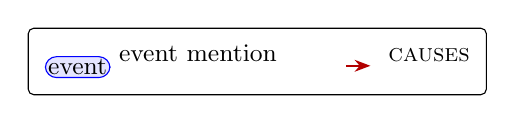
\begin{tikzpicture}
\node[draw, fill=white, font=\small, anchor=north,
      inner sep=6pt, rounded corners=2pt] {%
  \tikz[baseline=-0.5ex]{\node[draw=blue, fill=blue!10,
    rounded corners, inner sep=1pt, font=\small]{event};} event mention
  \qquad
  \tikz[baseline=0.4ex]{\draw[-{Stealth[length=2mm]}, thick, red!70!black, shorten <=3pt, shorten >=3pt](0,0)--(1.6em,0);}  \textsc{causes}%
};
\end{tikzpicture}

\caption{Annotated example from EventStoryLine~0.9 (\texttt{3\_7ecbplus.xml}). Blue boxes are event mentions. Arrows show \textsc{causes} relations.}
\label{fig:3-7ecbplus-xml}
\end{figure}

\end{document}
